\section{Results}\label{sec:results}

We apply our method to another set of mock data, the spherical models
for the Gaia challenge by Walker and Penarrubia. They consist of
dynamical tracer populations with density distribution

\begin{equation}
\nu_*(r) = \nu_0\left(\frac{r}{r_*}\right)^{-\gamma_*} \left[1+\left(\frac{r}{r_*}\right)^{\alpha_*}\right]^{(\gamma_*-\beta_*)/\alpha_*}
\end{equation}

inside dark matter halos of the form

\begin{equation}
\rho_{\text{DM}} = \rho_0\left(\frac{r}{r_{\text{DM}}}\right)^{-\gamma_{\text{DM}}}\left[1+\left(\frac{r}{r_{\text{DM}}}\right)^{\alpha_{\text{DM}}}\right]^{(\gamma_{\text{DM}}-\beta_{\text{DM}})/\alpha_{\text{DM}}}
\end{equation}

with scale radii $r_*, r_\text{DM}$, inner and outer logarithmic
slopes of $\gamma_*, \gamma_{\text{DM}}$ and
$\beta_*,\beta_{\text{DM}}$, with transition parameters $\alpha_*,
\alpha_{\text{DM}}$.

The anisotropy follows the functional form of \citet{Osipkov1979} and
\citet{Merritt1985},

\begin{equation}
\beta_{\text{anisotropy}}(r)=1-\frac{\sigma_\theta^2}{\sigma_r^2} = \frac{r^2}{r^2+r_a^2}.
\end{equation}

with scale radius $r_a$, turning over from nearly isotropic at $r\to
0$ to radially isotropic at $r_*=r_a$.

Of these distributions, finite samplings are taken and converted to
mock observational data including spectral indices, systemic
velocities, proper motions, binary motion.


\subsection{Cusps and Cores}

Applied on a profile with a core in the DM density profile, our method
converges fast in the beginning, see fig. \ref{fig:cusp}.

\begin{figure*}
\begin{center}
\hspace{-7mm}
%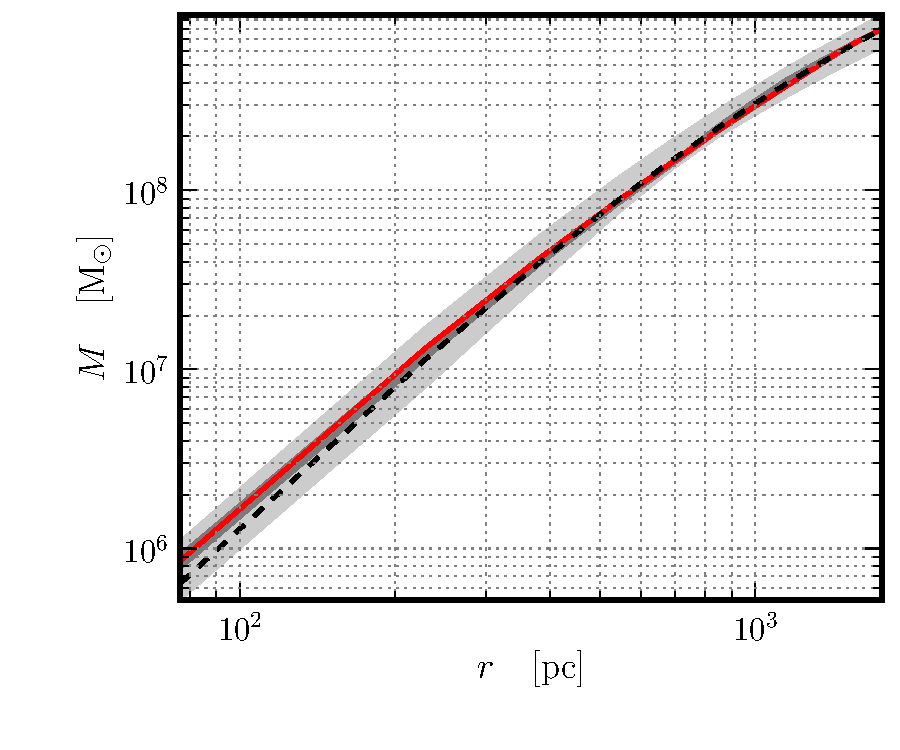
\includegraphics[width=0.5\textwidth]{fig/1000its.pdf}
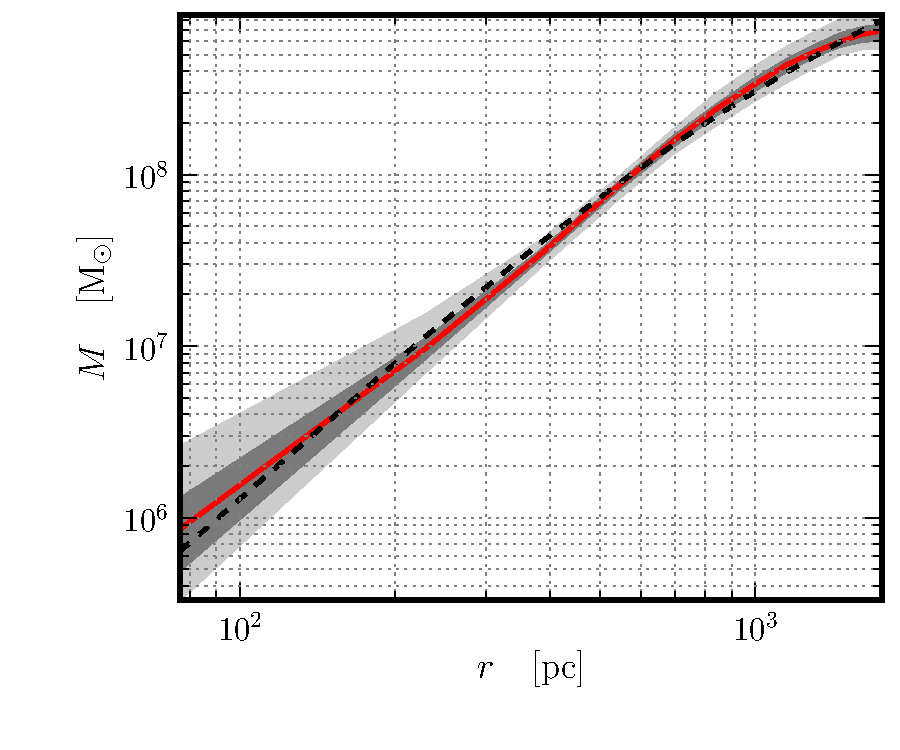
\includegraphics[width=0.5\textwidth]{fig/recent_50k.pdf}
\caption{Reconstructed mass of a cusped model (red shows median,
  shaded areas are 68 and 90 percentiles) for $10^4$ tracer particles,
  after 50000 iterations. The black dashed curve shows the underlying
  theoretical model.}
\label{fig:cusp}
\end{center}
\end{figure*}

If run for 50000 iterations, the profile in the right plot emerges,
with broader errorbars and a slight mismatch above $r_{vir}=1000{\rm
  pc}$.

The model is best constrained around $r=500$pc, which corresponds to
the scale radius of both the stellar tracers.

For a cored profile, we have a similar result, see fig. \ref{fig:core}.

\begin{figure*}
\begin{center}
\hspace{-7mm}
%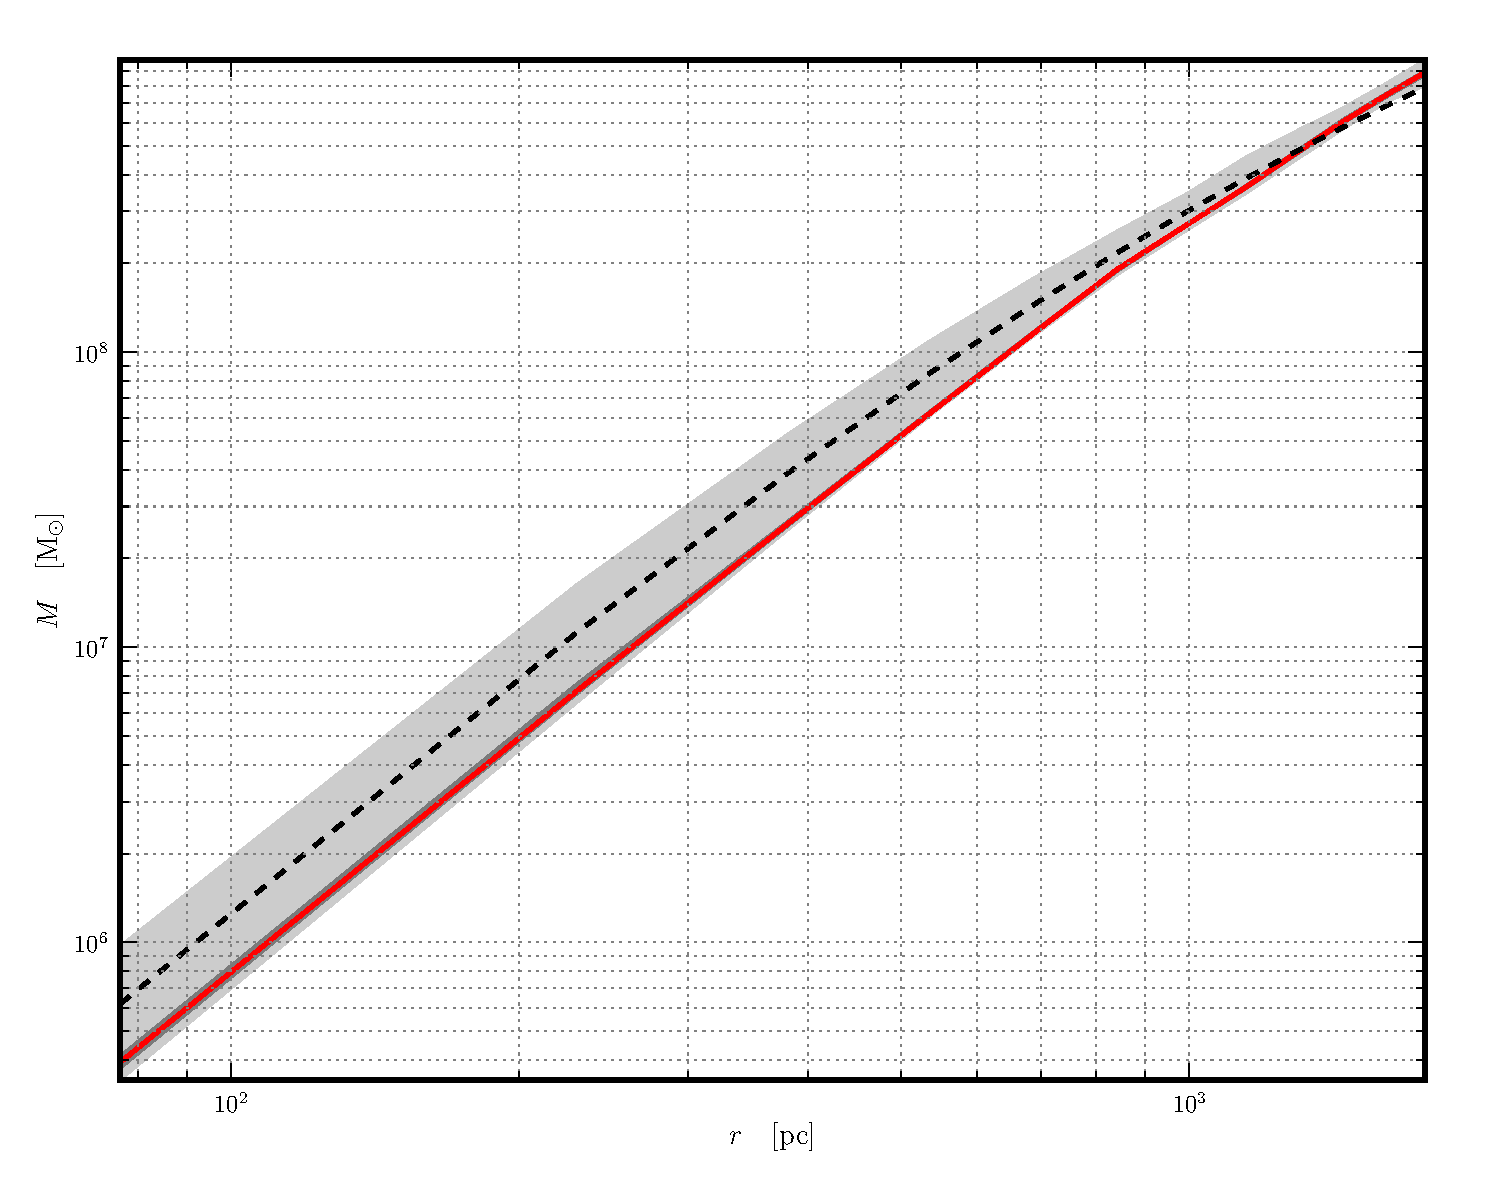
\includegraphics[width=0.5\textwidth]{fig/core_2k.pdf}
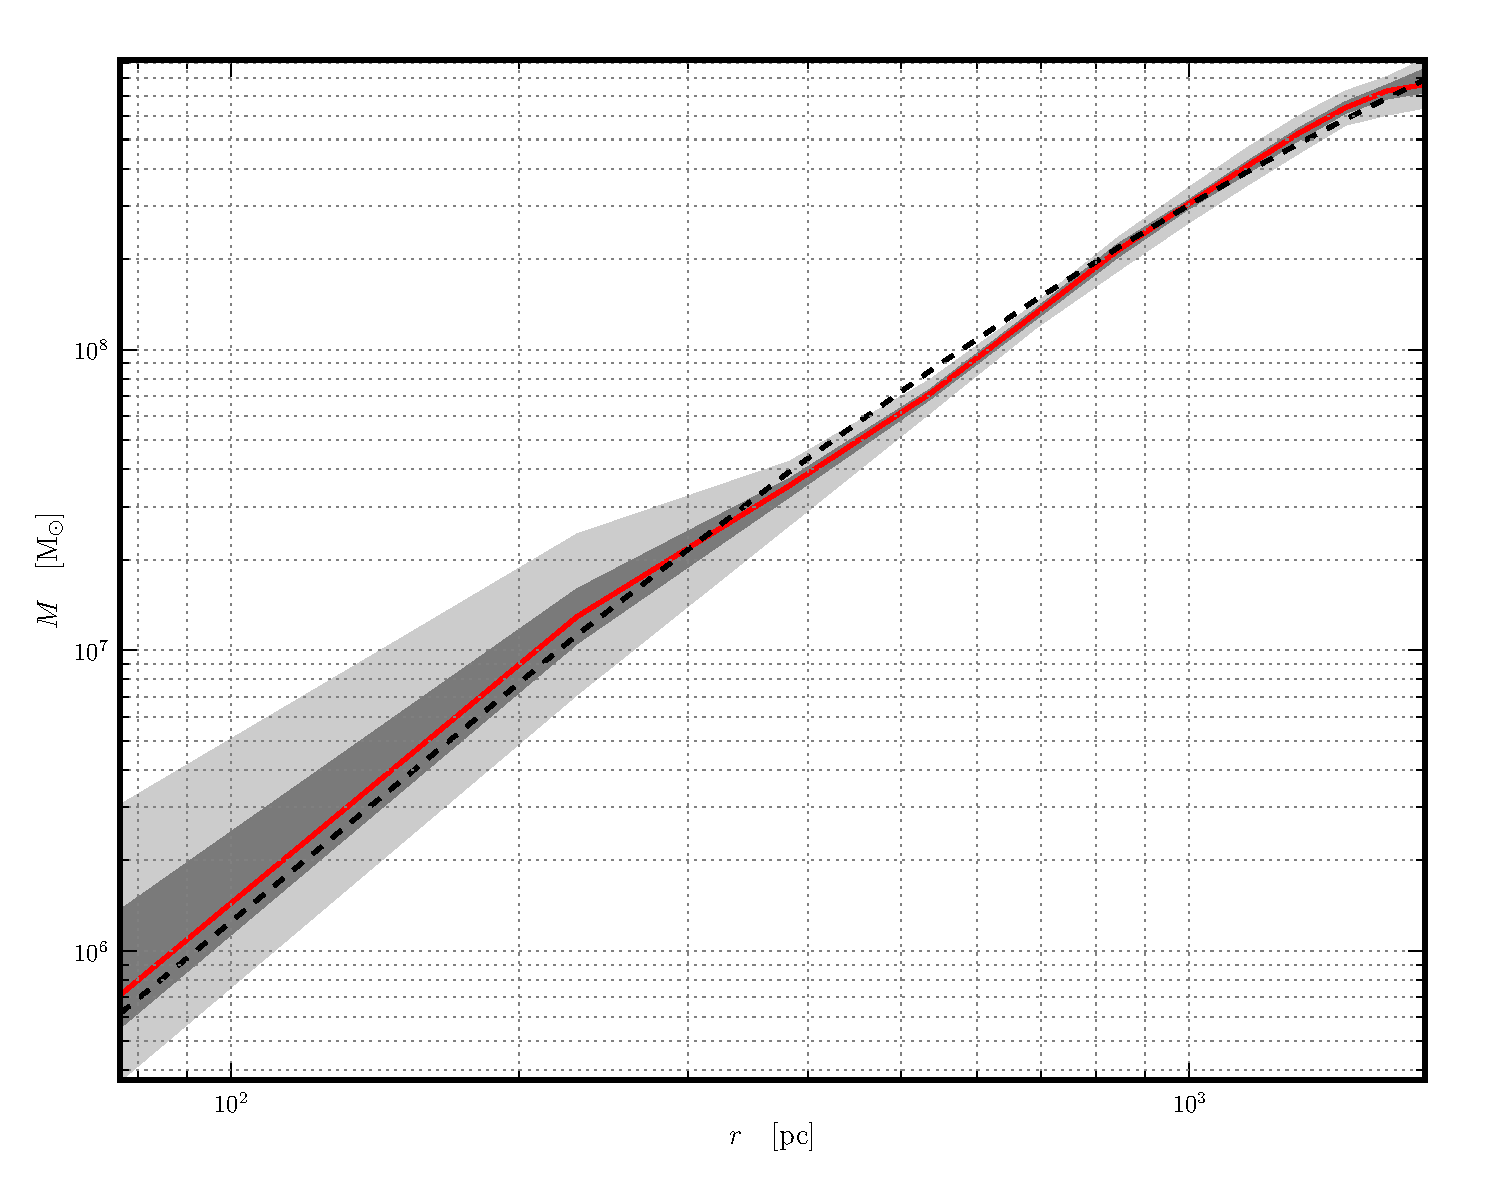
\includegraphics[width=0.5\textwidth]{fig/core_30k.pdf}
\caption{A cored profile: Reconstructed mass of the MCMC model (red
  shows median, shaded areas are 68 and 90 percentiles) for $10^4$
  tracer particles after 30000 iterations. The black dashed curve
  shows the underlying theoretical model.}
\label{fig:core}
\end{center}
\end{figure*}

Best restrictions are around $500$pc again, only this time a little
too low.
